\chapter{Cosmological Evolution}
In this chapter we briefly describe the evolution of the Universe. For more comprehensive lectures see e.g. \cite{Ref:Weinberg}, \cite{2002col.luc..cosmology} or \cite{2010deto.book.....A}. We begin with basic equations for the evolution and apply them to cosmological scales. We describe different epoch in history of the Universe and also introduce number of cosmic distances often used to put observational constraints on dark energy. We show some fundamental issues with the simplest models -- horizon problem, missing (dark) matter and accelerated expansion of the Universe -- and arrive to concordance \LCDM\ model. We describe background evolution and formation of structures in \LCDM\ model and introduce some basic observables. At the end of the chapter we outline some issues with the cosmological constant and offer some basic alternative in modified gravity models.

\section{Background evolution}
Standard cosmological model is based on the \textit{cosmological principle}. The cosmological principle states that the Universe is homogeneous and isotropic on sufficiently large scales (beyond those traced by the large-scale structure of the distribution of galaxies). The cosmic microwave background (CMB) observations strongly support this statement as photons from different parts of the Universe are coming with almost identical temperatures. This isotropy, however, does not imply homogeneity. The \textit{Copernican Principle} states that the observer is not in a special place or time. With the observed isotropy the Copernican Principle implies the Cosmological Principle. The observed inhomogeneities and irregularities on local scales come from gravitational instability.
%%%%%%%%%%%%%%%%%%%%%%%
% Friedmann equations
%%%%%%%%%%%%%%%%%%%%%%%
\subsection{Friedmann equations}
The homogeneous and isotropic space-time is described by Friedmann-Lema\^{i}tre-Robertson-Walker (FLRW) metric given by
\eq{
    \label{eq:flrw}
    \dd s^2=g_\uv\dd x^\mu \dd x^\nu=-\dd t^2+a^2(t)\left[\frac{\dd r^2}{1-Kr^2} + r^2\left(\dd\theta^2+\sin^2\theta\dd\phi^2 \right) \right]\,,
}
where $g_{\mu\nu}$ is a metric tensor, $a(t)$ is a scale factor with cosmic time $t$ and $K=+1,-1,0$ is a curvature that corresponds to closed, open, and flat geometries. The scale factor can be arbitrary rescaled and we adopt the common normalization $a_0=1$. We can also transform \autoref{eq:flrw} to a more convenient form by setting $r=\sin\chi\ (K=+1),r=\chi\ (K=0)$, and $r=\sinh\chi\ (K=-1)$. The FLRW metric is then given by
\eq{
    \label{eq:flrw_chi}
    \dd s^2=-\dd t^2+a^2(t)\left[\dd \chi^2 + f_K^2(\chi)\left(\dd\theta^2+\sin^2\theta\dd\phi^2 \right)\right]\,,
}
where
\eq{
    f_K(\chi)=
    \begin{cases}
        \sin\chi & (K=+1)\,, \\
        \chi & (K=0)\,, \\
        \sinh\chi & (K=-1)\,.
    \end{cases}
}
By allowing taking the limit $K\to0$ we can rewrite $f_K(\chi)$ in a unified way
\eq{
    \label{eq:f_K}
    f_K(\chi)=\frac{1}{\sqrt{-K}}\sinh{(\sqrt{-K})\chi}\,.
}
In addition to the cosmic time $t$, we also introduce the conformal time $\eta$ defined by
\eq{
    \eta\equiv\int{a^{-1}\dd t}\,.
}
The dynamical equations of motion in the expanding Universe can be derived from the Einstein equations resulting in the Friedmann equations
\eq{
    \label{eq:Friedmann}
    H^2 &= \frac{8\pi G}{3}\rho - \frac{K}{a^2}+\frac{\Lambda}{3}\,, \\
    \frac{\ddot a}{a} &= -\frac{4\pi G}{3}(\rho + 3p)+\frac{\Lambda}{3}\,,\\
    \dot\rho &= -3H(\rho+p)\,,
}
where $H\equiv\dot a/a$ is the Hubble parameter, $\Lambda$ the cosmological constant, $\rho(t)$ is energy-density and $p$ pressure. We will be also using the conformal Hubble quantity
\eq{
    \mathcal{H}\equiv\frac{1}{a}\frac{\dd a}{\dd\eta}=Ha\,.
}
These three equations are not independent and we need to also specify the equation of state, $\rho=\rho(p,t)$. The first equation is usually also written in the form
\eq{
    \Omega_m+\Omega_\gamma+\Omega_K+\Omega_\Lambda=1\,,
}
where
\eq{
    \Omega_m\equiv\frac{8\pi G\rho_m}{3H^2}\,,\hspace{3pt}
    \Omega_\gamma\equiv\frac{8\pi G\rho_\gamma}{3H^2}\,,\hspace{3pt}
    \Omega_K\equiv-\frac{K}{a^2H^2}\,,\hspace{3pt}
    \Omega_\Lambda\equiv\frac{\Lambda}{3H^2}
}

Most matter species in the Universe can be described by a simple equation of state
\eq{
    p=\omega\rho\,,
}
where $\omega$ is constant. This lead to the following solutions in flat universe
\eq{
    \rho\propto a^{-3(1+\omega)}\,,\hspace{6pt}a\propto (t-t_i)^{2/(3(1+\omega)))}\,,
}
where $t_i$ is an integration constant. Relativistic matter has the equation of state $\omega=1/3$ and the cosmic evolution during the radiation-dominated epoch is given by $\omega\propto a^{-4}$ and $a\propto(t-t_i)^{1/2}$. Non-relativistic matter has negligible pressure $(\omega=0)$ and the evolution during the matter- dominated era is given by $\omega\propto a^{-3}$ and $a\propto(t-t_i)^{2/3}$.

The accelerated expansion of the Universe $(\ddot a>0)$ is possible only for $\omega<-1/3$ (see \autoref{eq:Friedmann}), i.e. negative pressure. Note that in Newtonian gravity there is no such equivalent. The pressure is related to a force associated with a local potential that depends on the position in space but in homogeneous and isotropic universe there is no such potential.

When $\omega=-1$, the energy-density $\rho$ is constant and corresponds to the cosmological constant. This energy-density connected to the cosmological constant is
\eq{
    \rho_\Lambda=\frac{\Lambda}{8\pi G}\,.
}
With constant energy-density the Friedmann equations lead to an exponential expansion $a\propto\exp{Ht}$.

%%%%%%%%%%%%%%%%%%%%%%%
% Hubble`s law
%%%%%%%%%%%%%%%%%%%%%%%
\subsection{Hubble`s law}
During the 1920s astronomers Slipher and Hubble found that the observed wavelength $\lambda_o$ of absorption lines of distant galaxies is larger than the wavelength $\lambda$ in the rest frame \cite{1929PNAS...15..168H}. This is due to the fact that the wavelength is stretched in proportion to the scale factor in an expanding Universe. The redshift $z$ is defined as
\eq{
    z\equiv\frac{\lambda_0}{\lambda} - 1=a^{-1}-1\,.
}
In an expanding Universe a physical distance $r$ from an observer (at the origin) to an object is given by $r=a(t)x$, where $x$ denotes the comoving distance. For objects which are motionless with respect to the Hubble flow the comoving distance remains constant. Taking the time derivative of $r$ we obtain
\eq{
    v_H\equiv\dot r=Hr+a\dot x
}
Because of the cosmic expansion, more distant objects are moving faster from us with velocity $v_H$. On the other hand, the peculiar velocity $v_p\equiv a\dot x$ describes the movement of an object with respect to the local Hubble flow. For small peculiar velocities and near objects $(z\ll1)$ we obtain
\eq{
    v\sim H_0r\,,
}
which is the law Hubble reported in 1929 by plotting the recessional velocity $v$ versus the distance $r$. His measurements were noisy but the current measurements give the Hubble constant the value \cite{collaboration2018planck}.
\eq{
    H_0=(67.4\pm0.5)\rm{\ km\ s}^{-1}\rm{Mpc}^{-1}
}

%%%%%%%%%%%%%%%%%%%%%%%
% Cosmic distances
%%%%%%%%%%%%%%%%%%%%%%%
\subsection{Cosmic distances}
In the expanding Universe there are many ways to specify the distance between two points due to the constantly changing distances and the fact that observers look back in time as they look out in distance.
\subsubsection{Comoving distance}
The light traveling along the $\chi$ direction satisfies the geodesic equation $\dd s^2=-\dd t^2+a^2(t)\dd \chi^2=0$. The light emitted at the time $t=t_1$ with $\chi=\chi_1$ (redshift $z$) reaches an observer at time$t=t_0$ with $\chi=0$ (redshift $z=0$). Integrating the geodesic equation
\eq{
    \label{eq:d_c}
    d_c\equiv\chi_1=\int_0^{\chi_1}\dd\chi=-\int_{t_0}^{t_1}\frac{\dd t}{a(t)}=\frac{1}{H_0}\int_0^z\frac{\dd\tilde z}{E(\tilde z)}\,,
}
where
\eq{
    E(z)\equiv H(z)/H_0=\sqrt{\Omega_{\gamma,0}(z+1)^4+\Omega_{m,0}(z+1)^3+\Omega_{K,0}(z+1)^2+\Omega_{\Lambda,0}}\,.
}
If we expand $E(z)$ around $z=0$ we can write the cosmic distance as
\eq{
    d_c=\frac{1}{H_0}z-\frac{E'(0)}{2H_0}z^2+\frac{2E'(0)^2-E''(0)}{6H_0}z^3+\mathcal{O}(z^4)\,,
}
where a prime represents a derivative with respect to $z$.
\subsubsection{Luminosity distance}
The luminosity distance $d_L$ is used in supernovae observations in order to link the supernova luminosity with the expansion rate of the Universe. It is defined by
\eq{
    d_L^2\equiv\frac{L_s}{4\pi F}\,,
}
where $L_s$ is the absolute bolometric (i.e., integrated over all frequencies) luminosity of a source and $F$ is the observed bolometric flux. The flux is defined by $F=L_0/S$, where $L_0$ is the observed luminosity and $S=4\pi f_K^2(\chi)$ is the area of a sphere at $z=0$.

The absolute luminosity is defined as energy emitted per unit time interval, $L=\Delta E/\Delta t$. The energy of a photon is inversely proportional to its wavelength, $E\propto\lambda^{-1}\propto 1+z$, which is stretching in an expanding universe. Also the time between arrival of two photons is proportional to the wavelength, $\Delta t\propto\lambda\propto(1+z)^{-1}$. The ratio $L_s/L_0$ is then
\eq{
    \frac{L_s}{L_0}=\frac{\Delta E_1}{\Delta E_0}\frac{\Delta t_0}{\Delta t_1}=(1+z)^2\,,
}
and the luminosity distance is
\eq{
    d_L=f_K(\chi)(1+z)\,.
}
Using \autoref{eq:f_K} and \autoref{eq:d_c} we can express $d_L$ as
\eq{
    \label{eq:luminosity}
    d_L=\frac{1+z}{H_0\sqrt{\Omega_{K,0}}}\sinh{\left(\sqrt{\Omega_{K,0}}\int_0^z{\frac{\dd\tilde z}{E(\tilde z)}}\right)}\,.
}
For small $z$ we can once again expand the expression and get
\eq{
    d_L=\frac{1}{H_0}z-\frac{E'(0)-2}{2H_0}z^2+\frac{2E'(0)^2-3E'(0)-E''(0)+\Omega_{K,0}}{6H_0}z^3+\mathcal{O}(z^4)\,.
}
\subsubsection{Angular diameter distance}
The angular diameter distance $d_A$ is defined as
\eq{
    d_A\equiv\frac{\Delta x}{\Delta\theta}\,,
}
where $\Delta\theta$ is the angle that subtends an object of actual size$\Delta x$ orthogonal to the line of sight. Whenever we look at objects of known size such as CMB anisotropies or BAO scale we use this distance.

The observer measures the size $\Delta x$ along the surface of a sphere with radius $\chi$ and from \autoref{eq:flrw_chi} follows
\eq{
    \Delta x=a(t)f_K(\chi)\Delta\theta\,.
}
The angular diameter distance is then
\eq{
    \label{eq:angular}
    d_A=a(t)f_K(\chi)=\frac{1}{1+z}\frac{1}{H_0\sqrt{\Omega_{K,0}}}\sinh{\left(\sqrt{\Omega_{K,0}}\int_0^z{\frac{\dd\tilde z}{E(\tilde z)}}\right)}\,.
}
Comparing \autoref{eq:angular} and \autoref{eq:luminosity} we can see that luminosity distance and the angular diameter distance have following relation
\eq{
    d_A=\frac{d_L}{(1+z)^2}\,.
}
\subsubsection{Degeneracy of the distance measurements}
We can se that up to the first order all the distances are the same and reduce to the Euclidean distance and that the Hubble`s law holds. With the increasing redshift the Hubble`s law dos not hold exactly and also different distances behave differently. This can be used to measure different properties of the Universe.

As the distances depend on the cosmological parameters through the integral $\int_0^z{\dd\tilde z/E(\tilde z)}$ and through $\Omega_K$ we can measure only those parameters contained in $E(z)$. Moreover, if we had distance measurements only around one particular redshift $z$ any combination of parameters that would produce similar $E(z)$ would be equally acceptable. This degeneracy can be broken by combination of measurements across different redshifts or by using other cosmological probes.

% \subsection{Very early universe}

% \subsubsection{Horizon problem}


%%%%%%%%%%%%%%%%%%%%%%%
% Formation and evolution of LSS
%%%%%%%%%%%%%%%%%%%%%%%
\section{Formation and evolution of LSS}
So far we have considered only equations for smooth, homogeneous and isotropic background. In order to describe the real Universe with its rich structures we must employ perturbation theory for cosmological equations.
\subsection{Newtonian gauge}
We will consider first order (linear) perturbations of the metric:
\eq{
    g_{\mu\nu}=g_{\mu\nu}^{(0)}+\delta g_{\mu\nu}\,,
}
where $g_{\mu\nu}^{(0)}$ is the FLRW metric \autoref{eq:flrw} and all the entries in the perturbed metric $\delta g_{\mu\nu}$ have to be small with respect to the background metric. The general perturbed metric can be written as
\eq{
    \delta g_{\mu\nu}=a^2(\eta)
    \begin{pmatrix}
        -2\Psi & w_i \\
        w_i & 2\Phi\delta_{ij}+h_{ij} \\
    \end{pmatrix}\,,
}
where $\Psi(t,x)$ and $\Phi(t,x)$ are spatial scalars, $w_i(t,x)$ is 3-vector, and $h_{ij}(t,x)$ is a traceless 3-tensor. We have a freedom to choose coordinates in which we will describe the equations of motion -- we can choose our \textit{gauge}. We wish to keep our background metric $g_{\mu\nu}^{(0)}$ the same (i.e. FLRW) and only change $\delta g_{\mu\nu}$. Note that unlike ordinary coordinate transformations a gauge transformation (although expressed as a change of coordinates) does not link different observers in the same spacetime but it links two different spacetimes seen by the same observer. For a detailed discussion of gauge choices, see e.g. \cite{PhysRevD.40.1804,10.1143/PTPS.78.1,PhysRevD.22.1882}.

We will choose to attach the observers to the points in the unperturbed frame, the so called \textit{Newtonian} or \textit{longitudinal} or \textit{shear-free} gauge. In this case the observer will detect a velocity field of particles falling into the clumps of matter and will measure a gravitational potential. We can impose up to four conditions on the metric, which corresponds to the four gauge coordinate transformations. The final perturbed metric is:
\eq{
    \label{eq:flrw_pert}
    \dd s^2=a^2(\eta)\left[-(1+2\Psi)\dd\eta^2+(1+2\Phi)\delta_{ij}\dd x^i\dd x^j\right]\,.
}
\subsection{Linear perturbations}
We now decompose the Einstein tensor and the energy-momentum tensor into background and perturbed parts. The background cosmological evolution is obtained by solving the zero-th order Einstein equations and is given by the Friedmann equations. The first order equations are given by the perturbation of the Einstein tensor, i.e. by perturbing the metric \autoref{eq:flrw_pert}, and by the perturbed energy-momentum tensor. The four-velocity $u^\mu$ is up to the first order
\eq{
    u^\mu\equiv\dddd{x^\mu}{\tau}=\left[\frac{1}{a}(1-\Psi),\frac{v^i}{a} \right]\,,
}
where $\tau$ is the proper time and $v^i=\dd x^i/\dd\eta$ is the matter peculiar velocity with respect to the general expansion.

The first order equations are (for details, see e.g. \cite{2002col.luc..cosmology,10.1143/PTPS.78.1}).
%%%%%%%%%%%%%%%%%%%%%%%
% Cosmological observables
%%%%%%%%%%%%%%%%%%%%%%%
\section{Cosmological observables}
Here we present a brief description of cosmological probes which will be used when constraining dark energy. For more details see e.g. \cite{DE_probes} or \cite{DE_probes2}.
%In shear-shear tomography, the shear of background galaxies, binned in redshift, is cross correlated. 
%\ssec{Introduction}
%http://terapix.phys.cmu.edu/misc/desc\_feb\_2015\_de\_school\_ShirleyHo.pdf \\
%https://sites.google.com/site/cmucosmos13/lecture-notes \\
%http://arxiv.org/pdf/1201.2434v2.pdf \\
\subsection{Supernovae}
Supernovae (SNe) are the most straightforward tool for studying cosmic acceleration, as they directly discovered the acceleration in the first place \cite{riess}. Type Ia supernovae (SNe Ia) are exploding stars defined by the lack of hydrogen and the presence of silicon in their early-time spectra \cite{SN}, and are a product of a thermonuclear explosion of a C/O white dwarf. Observations show that SNe Ia have a luminosity peak that is tightly correlated with the shape of their light curves -- supernovae that rise and fall more slowly have higher peak luminosity (first quantified by \cite{SN_lum}). From observations of (multiband) light curve shapes and colors the luminosity at a brightness peak can be predicted.

To measure cosmic expansion with Type Ia SNe, the observed flux and predicted luminosity are compared. From that the supernova's luminosity distance can be measured. An accurate redshift is obtained by measuring the host galaxy (calibrator). Since the distances to the local calibrators are usually determined from the Hubble expansion, this method gives the luminosity distance $D_L$ in units of $h\mins$ Mpc. Measured relation is used to constraint dark energy parameters.

Long-term task of the SN working group within DESC is \textit{Develop theoretical/numerical/empirical SN models to better describe or
improve the distance indicator}.
\subsection{Baryonic acoustic oscillations}
Baryonic acoustic oscillations (BAO) provide an entirely independent way of measuring cosmic distance. Sound waves propagating before recombination imprint a characteristic scale on matter clustering. The acoustic length scale can be computed as
\eq{
r_s=\int_0^{t_\ast}{\frac{c_s(t)}{a(t)}\dd t}=\int_{z_\ast}^{\infty}{\frac{c_s(z)}{H(z)}\dd z},
}
where asterisk denotes time (redshift) at recombination and $c_s$ is the sound speed. The behavior of $H(z)$ depends on the ratio of the matter density to radiation density and the sound speed depends on the ratio of radiation pressure to the energy density of the baryon-photon fluid, determined by the baryon-to-photon ratio. Both the matter-to-radiation ratio and the baryon-to-photon ratio can be measured from the CMB anisotropy power spectrum. This gives $r_s\sim150$ Mpc. The scale of the acoustic feature is stable to better than 1\% accuracy, making it an excellent standard ruler.

This effect can be detected in the angular clustering of galaxies in bins of photometric redshift, yielding the angular diameter distance. Furthermore, measuring the BAO scale in a velocity separation allows a direct determination of $H(z)$. The BAO method measures $D(z)$ in absolute units -- Mpc not $h\mins$ Mpc like SNe measurements, and thus BAO measurements to the same redshift carry different information. At low redshift $(z\lesssim0.5)$, the BAO method strongly complements SN measurements, while at higher redshift $(z\gtrsim0.5)$ the BAO method is an powerful probe of dark energy and cosmic geometry.
\subsection{Weak lensing}
Gravitational lensing is the deflection of light from distant sources due to the bending of space-time by baryonic and dark matter (lenses) along the line of sight (more about lensing in \autoref{appen-lens}). It is a very useful cosmological probe because it is sensitive to all matter regardless of its nature. In the limit of very small deflection angles it is called weak lensing (WL). WL causes tiny distortions ($\sim0.5\%$), or ``shear'', in galaxy sizes and shapes -- see \autoref{fig_WL_Abell}. Intrinsic size or shape of a given galaxy are unknown, but normally, galaxy orientations are assumed to be random ($\sim30\%$ dispersion), so they should not exhibit statistically significant and coherent alignments. In the presence of lensing, small but coherent shears in background galaxy images are induced. This means that WL is statistically detectable by averaging shapes over many lensed galaxies. In principle either the shearing of galaxies (shape distortion) or their magnification (size distortion) can be measured. However, in practice the shape distortions is used much more widely, since the scatter in shapes of galaxies is less than the scatter in their sizes.

Weak lensing provides a direct measure of the distribution of matter, independent of any assumptions about galaxy biasing\footnote{Galaxy bias is the difference in the distribution of galaxies and that of the underlying dark matter. The biasing factor $b$ is defined such that the relative fluctuations in the spatial number density of galaxies are $b$ times the relative density fluctuations.}. Since this distribution can be predicted theoretically, and its amplitude can be directly used to constrain cosmology, weak lensing has great potential as a cosmological probe. The correlation of the density field of nearby galaxies with the lensing shear measured on more distant galaxies is called \textit{galaxy-galaxy lensing}. Most lens systems involve sources (and lenses) at moderate or high redshift, and thus can lensing probe the geometry of the Universe -- the measurement of the shear correlation function as a function of the redshifts of observed galaxies is called \textit{tomography}. The scaling of the galaxy-galaxy lensing signal as a function of the source redshift, known as \textit{cosmography}, depends purely on geometric factors and hence can be used to construct a distance-redshift relation.

Long-term tasks of the WL working group within DESC are \textit{Develop non-canonical WL statistics that have the potential to improve
dark energy constraints} and \textit{Extend WL data analysis methods from Stage III surveys to LSST}.
%%%%%%%%%%%%%%%%%%%
% TODO
%%%%%%%%%%%%%%%%%%%
% \begin{figure}
% 	\centering
% 		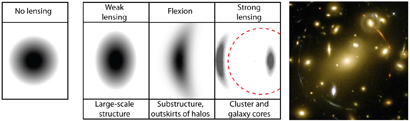
\includegraphics[scale=1.00]{img/WL_abel.jpg}
% 	\caption{(Left) Illustrations of the effect of a lensing mass on a circularly symmetric image. Weak lensing elliptically distorts the image, flexion provides an arc-ness and strong lensing creates large arcs and multiple images. (Right) Galaxy cluster Abell 2218, strongly lensed arcs can be seen in around the cluster. Every background galaxy is weakly lensed. From NASA, ESA, and Johan Richard (Caltech, USA).}
% 	\label{fig_WL_Abell}
% \end{figure}
\subsection{Large-scale structure}
Studying the large-scale structures (LSS) of the Universe is of a great importance for the cosmology. Since the clustering of matter on scales from galaxies to superclusters came from quantum fluctuations in the very early Universe with important modification by radiation and baryons, the LSS encode critical information about the contents of the Universe, the origin of the fluctuations, and the cosmic expansion background in which the structures evolved.

Measurements of large-scale power spectrum for the spatial distribution of matter as a function of redshift constrain the cosmic expansion history, the cosmological distance scale, the growth rate of structures, the mass of the neutrinos and the abundance of dark matter. This includes BAO measurement of the distance-redshift relation (as a standard ruler). The BAO with the growth of the LSS in the Universe form two robust probes of dark energy, and a potential discriminator between dark energy and modified gravity models. Beyond the dark energy, the large scale power spectrum is a probe of both neutrino mass and primordial non-gaussianity.

Long-term task of the LSS working group within DESC is \textit{Scalable optimal LSS analysis software development}.
\subsection{Galaxy clusters}
The observed number density and clustering of galaxy clusters as a function of mass and redshift provides a powerful toolset to constraining cosmology.  Galaxy clusters provided the first line of evidence for the existence of dark matter \cite{zwicky} and cluster mass-to-light ratio measurements suggested that the matter density in the universe was sub-critical \cite{Gott}. Galaxy clusters measurements are sensitive to both the expansion history and the growth of structure in the Universe enabling to distinguish between dark energy and modified gravity models for cosmic acceleration. Additional probes are measurements of the baryonic mass fraction in clusters, and of the tomographic lensing signatures through clusters.

The basic idea of cluster abundance studies is to compare the predicted space density of massive halos to the observed space density of clusters. The basic observables are the richness, the number of galaxies in a specified luminosity and color range. Halo abundance is sensitive to the amplitude of the matter power-spectrum $\sigma_8$\footnote{$\sigma_8$ is a linear fluctuation in the mass distribution on scales of $8h\mins$ Mpc} and the matter density $\Omega_m$, more precisely a combination of a form $\sigma_8\Omega_m^q$, with $q\approx0.4$ \cite{white}. The degeneracy between $\sigma_8$ and $\Omega_m$ can be broken by measuring abundances at a variety of masses.

Long-term task of the Cl working group within DESC is \textit{Optimizing magnification-based cluster mass calibration}.
\subsection{Strong lensing}
Strong gravitational lensing (SL) refers to the multiple imaging of a background object due to a massive foreground object (typically clusters of galaxies) -- see \autoref{fig_WL_Abell}. The resulting angular displacement, morphological distortion, and time delay can be used to measure dark energy parameters. Strong gravitational lensing time delays measure a combination of distances that combining with other dark energy probes can further constraint cosmological parameters. The time delays is also expected to test gravity on scales where the screening mechanisms is becoming active (more about screening mechanisms of modified gravities in \autoref{screen}).

Another independent way to measure dark energy parameters with SL is the analysis of systems with multiple sets of multiple images \cite{SL_in_CLGs}. The positions of these multiple images depend strongly on the detailed properties of the lens mass distribution and on the angular diameter distance ratios between the lens, source and observer, they encapsulate information about the underlying cosmology. This dependence on the geometry can be used to derive constraints on the cosmological parameters.

Long-term task of the SN working group within DESC is \textit{Explore multiple source plane cosmography as a competitive DE probe}.
\subsection{Redshift-space distortions}
%(and thus an apparent distance)
When we observe distant galaxies, two features determine their redshifts -- the Hubble expansion and their peculiar velocities. The peculiar velocities of galaxies thus cause them to appear displaced along the line of sight in redshift space. These displacements lead to redshift distortions in the pattern of clustering of galaxies in redshift space and make large scale galaxy clustering anisotropic. Redshift-space distortions (RSD) have the tremendous advantage of bearing information about the dynamics of galaxies. The strength of the anisotropy is governed by distortion parameter $\beta = f(z)/b(z)$, where $f(z)$ is the logarithmic growth rate of fluctuations. By modeling the full redshift-space galaxy power spectrum one can obtain combination of the product of the matter clustering amplitude and the growth rate.

Anisotropy of galaxy clustering offers an alternative to weak lensing and cluster abundances as a tool for measuring the growth of structures. RSD directly measure the rate at which structure is growing at the redshift of observation unlike WL and galaxy cluster measurements  which measure the rate of growth at multiple redshifts. RSD measurements can improve constraints on dark energy models and they can be used to constrain departures from GR by testing consistency of the growth and expansion histories. The key challenge in modeling RSD is accounting for nonlinear effects, including nonlinear or scale-dependent bias between galaxies and matter, at the level of accuracy demanded by the LSST`s precision.